\documentclass[main.tex]{subfiles}

\begin{document}
\section[intro]{Introduction\hypertarget{sec:intro}{}}
%%
%% The introduction is an overview of the main ideas used in your approach!
%%
To recognise and count the coins in an image, Coinsy, have three subtasks: 1) Image processing (includes image segmentation and smoothing), 2) Feature Extraction, and 3) Classifiation (and then counting the coins).

\begin{figure}[!t]
  \begin{subfigure}[t]{0.5\textwidth}
    \centering
    \resizebox{\linewidth}{!}{\subfile{./flowchart.trg.tex}}
    \caption{Operation pipeline to train Coinsy} \label{trgPipe}
  \end{subfigure}
  \begin{subfigure}[t]{0.5\textwidth}
    \centering
    \resizebox{\linewidth}{!}{\subfile{./flowchart.demo.tex}}
    \caption{Pipeline for (trained) Coinsy to count coins} \label{evalPipe}
  \end{subfigure}
  \caption{Differences in Pipeline; Yellow boxes indicates the image processing procedures; Blue indicates the feature extraction procedures; Violet indicates the classification procedures.} \label{trgVSeval}
\end{figure}

For Coinsy to be a proficient counter, we have to first train it. The processes that Coinsy goes through for training differs from evaluation as described in figure \autoref{trgVSeval}. We will describe her training in the next section - \hyperlink{method}{methodology}, and her \hyperlink{resut}{evaluation results} after. Lastly, we conclude with a \hyperlink{discussion}{discussion on Coinsy performance}.

In the following subsections, we give an overview of the operation pipeline for each subtasks. The approach here is an abstract idea of what we did for our base model. Additional techniques were explored and will be discussed in later section.

\subsection{Data} \label{sec:Data}
The data we were given are images (split into two dataset - \texttt{harder} and \texttt{simpler}) with objects in the foreground for us to classify. The objects differ in colors and some are very similar to the background - such as 1 pound coins (see \autoref{montage_data}). Hence, the classifier must be invariant to rotation of objects, and importantly to detect the objects will the images to be processed, such that the objects are salient to the computer vision. The real challenge lies in segmentation of the image.

\begin{figure}[!h]
  \centering
  \begin{subfigure}[b]{.3\textwidth}
    \centering
    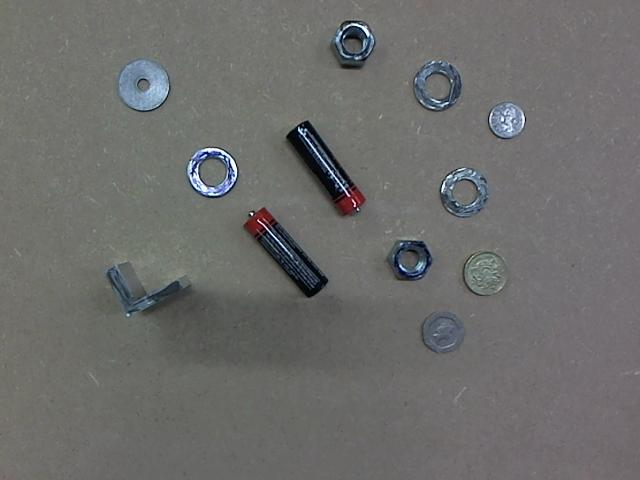
\includegraphics[width=\textwidth]{./img/sample_fig/02.jpg}
  \end{subfigure}
  \begin{subfigure}[b]{.3\textwidth}
    \centering
    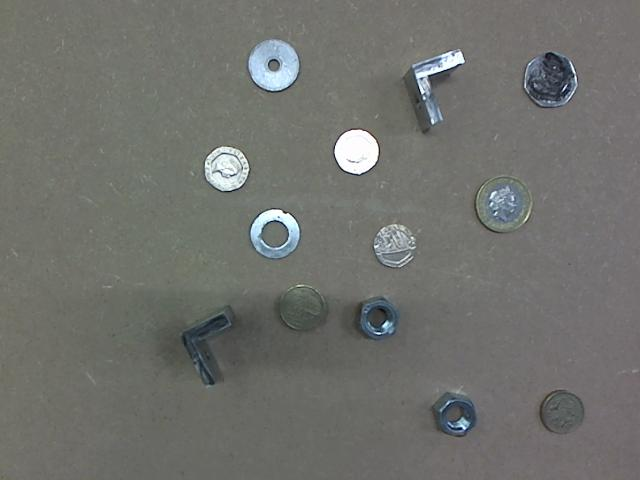
\includegraphics[width=\textwidth]{./img/sample_fig/04.jpg}
  \end{subfigure}
  \begin{subfigure}[b]{.3\textwidth}
    \centering
    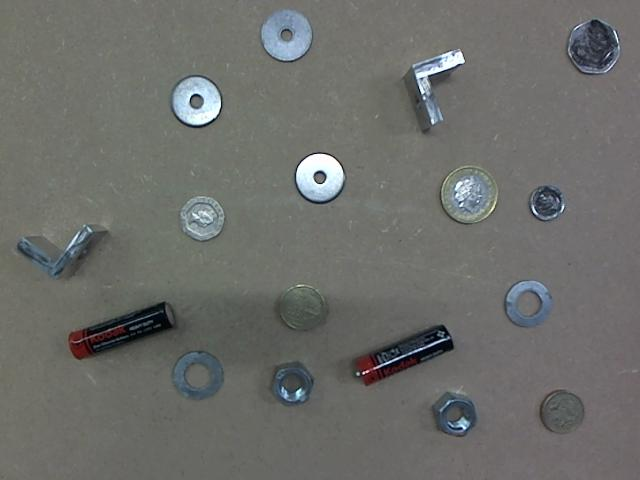
\includegraphics[width=\textwidth]{./img/sample_fig/03.jpg}
  \end{subfigure}
  \caption{Sample images from given data.}
  \label{montage_data}
\end{figure}
\begin{figure}[!h]
  \centering
  \begin{subfigure}[b]{.3\textwidth}
    \centering
    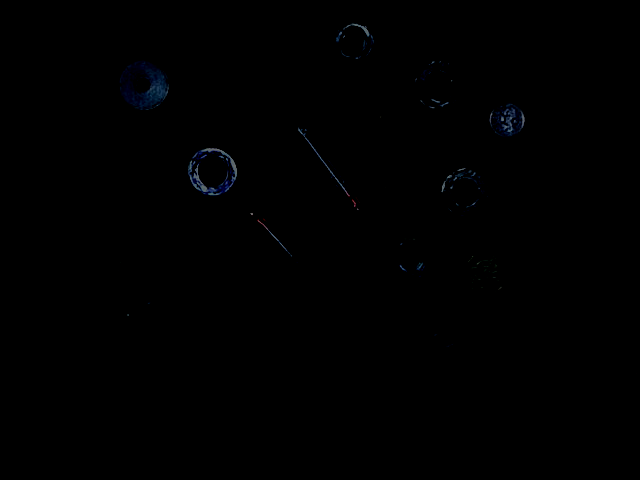
\includegraphics[width=\textwidth]{./img/bg_model/02_bgremove.png}
  \end{subfigure}
  \begin{subfigure}[b]{.3\textwidth}
    \centering
    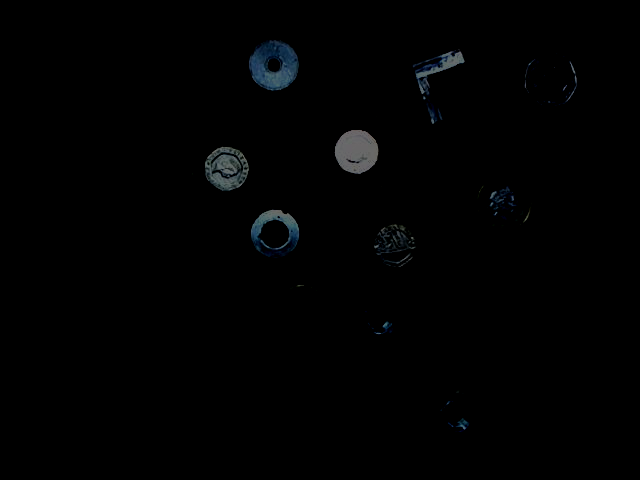
\includegraphics[width=\textwidth]{./img/bg_model/04_bgremove.png}
  \end{subfigure}
  \begin{subfigure}[b]{.3\textwidth}
    \centering
    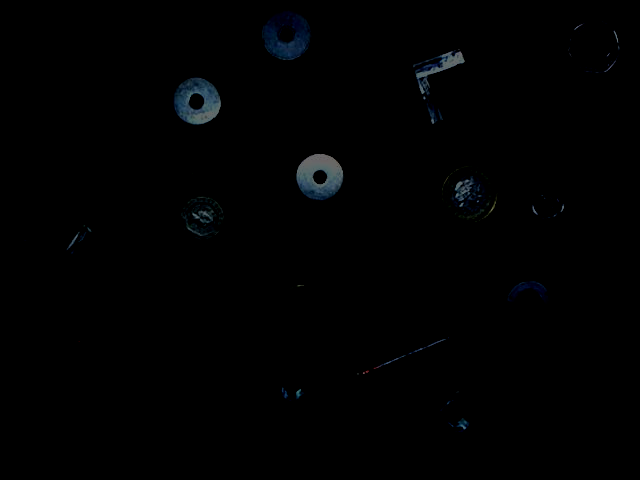
\includegraphics[width=\textwidth]{./img/bg_model/03_bgremove.png}
  \end{subfigure}
  \caption{Sample images after their background is subtracted.}
  \label{montage_data_bgremove}
\end{figure}

\subsection{Image Processing}
The image processing step aims to 1) make all images (for training the model or for evaluation) comparable, 2) extract objects in the foreground (also known as image segmentation). The outcome of this stage is an array of subimages ready for feature extraction.

The central idea is to, first, model the background before subtracting it from all images; second - make the edges of the objects 'obvious' by thresholding; third - crop out the objects to obtain the subimages. This is one of the many image segmentation technique available, and further exploration of other techniques is discussed later.

\subsubsection*{Background Subtraction}
In this coursework, since a background image is not readily available, we have to model it. Noting that images varies in illumination, we have to make the images comparable by normalising it first, using the following formula.
$$ P_{r,c}(R',G',B')=(\frac{R}{\sqrt(R^2+G^2+B^2)},\frac{G}{\sqrt(R^2+G^2+B^2)},\frac{B}{\sqrt(R^2+G^2+B^2)})$$

With objects scattered around randomly in the images, we find the median of all image pixels for each channel separately in order to reconstruct the background.

The outcome of the background with and without normalisation is shown in \autoref{bg_model}.

\begin{figure}[!h]
  \centering
  \begin{subfigure}[b]{.45\textwidth}
    \centering
    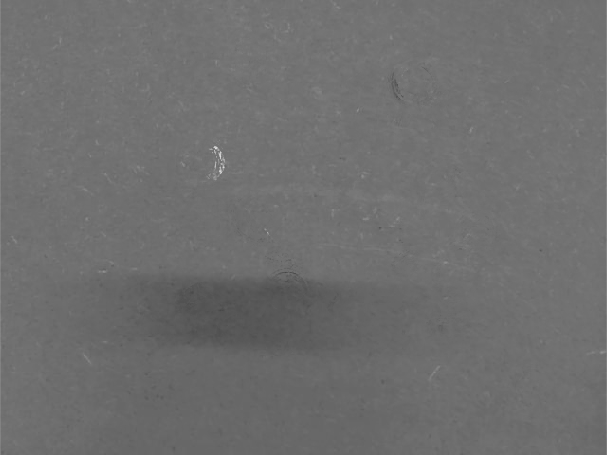
\includegraphics[width=\textwidth]{./img/bg_model/org_1.png}
    \caption{Background model without normalisation}
  \end{subfigure}
  \begin{subfigure}[b]{.45\textwidth}
    \centering
    
\includegraphics[width=\textwidth]{./img/bg_model/norm_1.png}
    \caption{Background model after normalisation}
  \end{subfigure}
  \caption{Background model generated from all 14 images}
  \label{bg_model}
\end{figure}


% Our approach is similar, but uses a neighbourhood of pixels around a target point. Hence, for a window of size 3, we have
% $bg\_model_{r,c} = median(i_{r+1,c+1}, i_{r+1,c}, i_{r+1,c-1},
%                           i_{r,c+1}, i_{r,c}, i_{r,c-1},
%                           i_{r-1,c+1}, i_{r-1,c}, i_{r-1,c-1}) $.
%
% The outcome of the background (with and without normalisation) are:
%
% \begin{figure}[!h]
%   \centering
%   \begin{subfigure}[t]{\textwidth}
%     \centering
%     \begin{subfigure}[t]{.3\textwidth} %% taking median
%         \centering
%         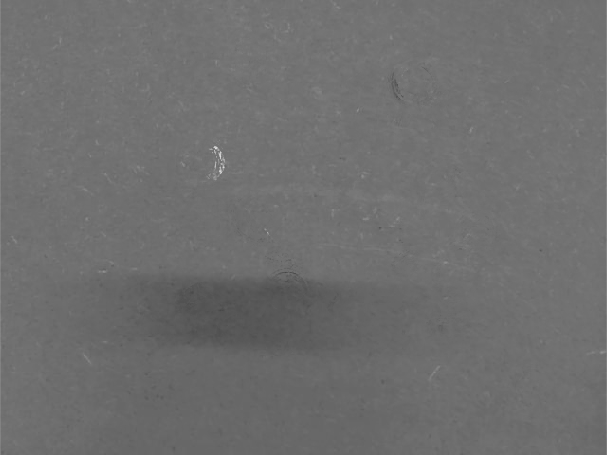
\includegraphics[width=\textwidth]{./img/bg_model/org_1.png}
%     \end{subfigure}
%     \begin{subfigure}[t]{.3\textwidth} %% window_size = 3
%         \centering
%         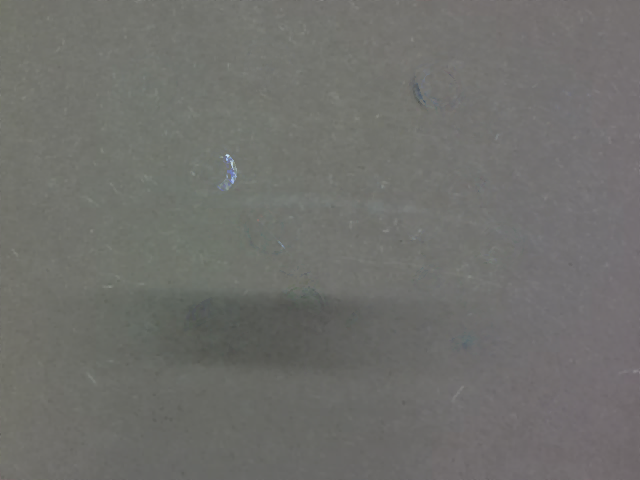
\includegraphics[width=\textwidth]{./img/bg_model/org_3.png}
%     \end{subfigure}
%     \begin{subfigure}[t]{.3\textwidth} %% window_size = 5
%         \centering
%         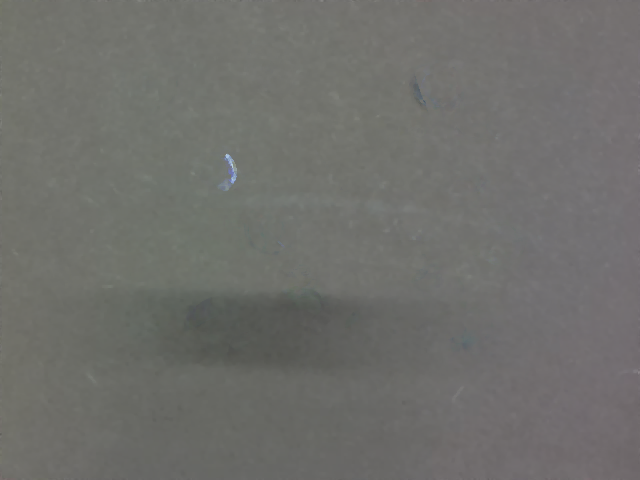
\includegraphics[width=\textwidth]{./img/bg_model/org_5.png}
%     \end{subfigure}
%   \end{subfigure} %% LOWER IMAGE - NORMALISED
%   \begin{subfigure}[b]{\textwidth}
%     \centering
%     \begin{subfigure}[t]{.3\textwidth} %% taking median
%         \centering
%         
\includegraphics[width=\textwidth]{./img/bg_model/norm_1.png}
%         \caption{Neighbouhood=1}
%     \end{subfigure}
%     \begin{subfigure}[t]{.3\textwidth} %% window_size = 3
%         \centering
%         
\includegraphics[width=\textwidth]{./img/bg_model/norm_3.png}
%         \caption{Neighbourhood=3}
%     \end{subfigure}
%     \begin{subfigure}[t]{.3\textwidth} %% window_size = 5
%         \centering
%         
\includegraphics[width=\textwidth]{./img/bg_model/norm_5.png}
%         \caption{Neighbourhood=5}
%     \end{subfigure}
%   \end{subfigure}
%   \caption{Sample images from given data.}
%   \label{montage_bg}
% \end{figure}


The sample images with their background removed is shown in \autoref{montage_data_bgremove}. It is evident that the background removal process removed the background - making the images appearing black. However, it also inevitably reduce the intensity for the bottom half of each images, such that the objects are no longer salient to our eyes. This is because the background we modelled have a lower intensity at the bottom, possibly due to presence of shadow in all 14 images.

Nevertheless, the historgram  is still bimodal, which is essential for thresholding to be effective.

\subsubsection*{Segmentation}



\subsection{Classification}



\end{document}
